\documentclass{article}
\usepackage{mathtools}
\usepackage{amsmath}
\usepackage{amssymb}
\usepackage{amsthm}
\usepackage{systeme}
\usepackage{newtxtext}
\usepackage{newtxmath}
\usepackage{listings}
\usepackage{xcolor}
\usepackage{array}
\usepackage{makecell}
\usepackage{booktabs}% http://ctan.org/pkg/booktabs
\usepackage{float}
\usepackage{hyperref}
\usepackage{tikz}
\usepackage{multicol}
\usepackage[utf8]{inputenc}
\usepackage[english]{babel}

\usetikzlibrary{arrows.meta}

\restylefloat{table}
\newcommand{\tabitem}{~~\llap{\textbullet}~~}

\newtheorem{theorem}{Theorem}[section]
\newtheorem{corollary}{Corollary}[theorem]
\newtheorem{defn}[theorem]{Deffinition}
\newtheorem{lemma}[theorem]{Lemma}
\newtheorem{axiom}[theorem]{Axiom}

\newcommand{\vVar}{\mathscr{v}_{var}}
\newcommand{\Var}{\mathbb{V}ar}
\newcommand{\vE}{\mathscr{v}}
\newcommand{\vBool}{\mathscr{v}_B}
\newcommand{\Ts}{\mathcal{T}_s}
\newcommand{\BranchConjunction}{%
\begin{align*}
			\bigwedge_{i=1}^{I} \; C(a_i, b_i) \:\: & \wedge \:\: 
			\bigwedge_{k=1}^{K} \; \neg C(e_k, f_k) \:\: \wedge \:\: \\
			\bigwedge_{j=1}^{J} \; d_j \neq 0 \:\: & \wedge \:\:
			\bigwedge_{l=1}^{L} \; g_l = 0 \:\: \wedge \:\:\\
			\bigwedge_{p=1}^{P} \; m_p \le_\mu n_p \:\: &\wedge \:\:
			\bigwedge_{q=1}^{Q} \; u_q <_\mu v_q \:\:
\end{align*}%
}

\lstset { %
    language=C++,
    backgroundcolor=\color{black!5}, % set backgroundcolor
    basicstyle=\footnotesize,% basic font setting
}

\title{Satisfiability Of Qualitative Contact Logics}
\date{2019-9-28}
\author{Martin Stoev}

\begin{document}
	\maketitle
	\newpage

	\tableofcontents

	\newpage

	\section{Tableaux Method}
Properties for a logical formula are best proven when the formula is decomposed into subformulas. Namely, the formula is defined in such a way that it can be described with a a structural recursive approach. The idea is to test a property only for some subformula and then to derive that property for the given formula.
Being able from a subformula to conclude properties for the formula itself leads to well structured and performant algorithms.

The Tableau method is a formal proof procedure and can be found in many variants. Formally, this procedure is used to refute the validity of formulas. Specifically, if a formula X is given and we want to prove that X is valid, then we construct a new formula that will represent the invalidity of X. This new formula is usually created with additional syntactic expressions. Proving that the newly created formula is not valid, it implies proof of the validity of X. The proofing process uses steps to break down the given formula into simpler formulas. If these steps are applied multiple times, the proof of the initial complex formula comes down to a proof using syntactic comparisons of basic formulas, where a basic formula is a formula which can not be decomposed further.

For our purposes, we will use a slightly different version of the method described above, namely with the help of the decomposition steps we will try to find a model with certain properties in which the given formula will not be valid.

		\subsection{Propositional logic tableau}
The tableau method for propositional logic comes down to defining the decomposition of the propositional logic operations $\{ \neg, \vee, \wedge, \rightarrow, \leftrightarrow \}$. To reach this goal we need to improve our syntactical arsenal, namely to add the ability for asserting the validity of a formula. In order to do this we shall introduce two signs. These signs when combined with a formula will assert whether the formula is true or false. Formally, the two signs are \{ T, F \}. Let $\varphi$ be a formula, then
\begin{itemize}
	\item T$\varphi$ - asserts the validity of the formula $\varphi$
	\item F$\varphi$ - asserts the invalidity of the formula $\varphi$
\end{itemize} 

The tableau of a formula $\varphi$ begins with F$\varphi$. The intuition behind it is that we start with an assertion that $\varphi$ is not valid in some model, and by decomposing the formula during the tableau process we seek for contradictions in the subformals. If such contradiction exists then the initial guess that the formula is not valid is not true meaning that the formula is valid. On the other hand if a contradiction does not exist then the formula is not valid, additionaly a model can be constructed in which the formula $\varphi$ is not valid.

The decomposition process is a set of tableau steps, which decompose the initial formula into basic formulas. A tableau step applies one of the tableau rules to slightly simplify the given formula. There are two rules for each operation in the logic. In the case of propositional logic with the following operations $\{ \neg, \vee, \wedge, \rightarrow, \leftrightarrow \}$ there are ten rules. Each rule decomposes the formula in at most two subformulas which depends on the arity of the operation. The decompositioning process forms a branch. A branch contains all signed subformulas which have been asserted in the decompositioning process.

A tableau rule which decomposes the formula in two subformulas may require the assertion of only one of the subformulas to be satisfied. In this case we will say that the branch is split into two branches. However in some terminologies this is noted as a new branch spawned from the original branch, or that two new branches are created . For the sake of simplicity we will use the terminology of branch splitting. In a scenario where the branch is split all asserted formulas in the branch are copied in the splitted branch together with the newly asserted subformula from the tableau rule.The newly asserted subformulas depend on the tableau rule.

	\subsubsection{Rules}
		\paragraph{Negation}
The rules for negations are straightforward. When a negation operation is encountered the sign of the captured formula changes.
		\newline
		\noindent\begin{minipage}{.5\linewidth}
		\begin{align*}
			\begin{array}{rl}
				& \mathbb{T}(\neg \varphi), X \\
				      \cline{2-2}
				      & \mathbb{F}(\varphi), X
			\end{array}
		\end{align*}
		\end{minipage}%
		\begin{minipage}{.5\linewidth}
		\begin{align*}
			\begin{array}{rl}
				& \mathbb{F}(\neg \varphi), X \\
			      \cline{2-2}
			      & \mathbb{T}(\varphi), X
			\end{array}
		\end{align*}
		\end{minipage}
		
		\paragraph{Conjunction}
This is a binary operation which means that the output of these rules is more complex than the negation rules.
The conjunction rule for a formula signed as valid decomposes the formula in two subformulas and assert the validity of both of them.
On the other hand the conjunction rule for a formula signed as invalid splits the branch into two branches and asserts the invalidity of the subformulas in each branch respectively.
		\newline
		\noindent\begin{minipage}{.5\linewidth}
		\begin{align*}
			\begin{array}{rl}
				& \mathbb{T}(\varphi \: \wedge \: \psi), X \\
			      \cline{2-2}
			      & \mathbb{T}\varphi, \mathbb{T}\psi, X
			\end{array}
		\end{align*}
		\end{minipage}%
		\begin{minipage}{.5\linewidth}
		\begin{align*}
			\begin{array}{rl}
				& \:\:\: \mathbb{F}(\varphi \: \wedge \: \psi), X \\
			      \cline{2-2}
			      & \mathbb{F}\varphi, X \:\:\:\:\:\:\:\: \mathbb{F}\psi, X
			\end{array}
		\end{align*}
		\end{minipage}

		\paragraph{Disjunction}
This is a binary operation which means that the output of these rules is more complex than the negation rules.
The disjunction rule for a formula signed as valid splits the branch into two branches and asserts the validity of the subformulas in each branch respectively.
On the other hand the disjunction rule for a formula signed as invalid decomposes the formula in two subformulas and assert the invalidity of both of them.
		\newline
		\noindent\begin{minipage}{.5\linewidth}
		\begin{align*}
			\begin{array}{rl}
				& \:\:\: \mathbb{T}(\varphi \: \vee \: \psi), X \\
			      \cline{2-2}
			      & \mathbb{T}\varphi, X \:\:\:\:\:\:\:\: \mathbb{T}\psi, X
			\end{array}
		\end{align*}
		\end{minipage}%
		\begin{minipage}{.5\linewidth}
		\begin{align*}
			\begin{array}{rl}
				& \mathbb{F}(\varphi \: \vee \: \psi), X \\
			      \cline{2-2}
			      & \mathbb{F}\varphi, \mathbb{F}\psi, X
			\end{array}
		\end{align*}
		\end{minipage}
		
		\paragraph{Implication}
The implication as well is a binary operation and depending on the asserting sign it decomposes the formula in two subformulas or splits into two separate branches.
		\newline
		\noindent\begin{minipage}{.5\linewidth}
		\begin{align*}
			\begin{array}{rl}
				& \:\:\: \mathbb{T}(\varphi \: \rightarrow \: \psi), X \\
			      \cline{2-2}
			      & \mathbb{F}\varphi, X \:\:\:\:\:\:\:\: \mathbb{T}\psi, X
			\end{array}
		\end{align*}
		\end{minipage}%
		\begin{minipage}{.5\linewidth}
		\begin{align*}
			\begin{array}{rl}
				& \mathbb{F}(\varphi \: \rightarrow \: \psi), X \\
			      \cline{2-2}
			      & \mathbb{T}\varphi, \mathbb{F}\psi, X
			\end{array}
		\end{align*}
		\end{minipage}
		
		\paragraph{Equivalence}
Both of the equivalence rules split the branch into separate branches, the details can be observed in the following equations.
		\newline
		\noindent\begin{minipage}{.5\linewidth}
		\begin{align*}
			\begin{array}{rl}
				& \:\:\:\:\:\:\:\: \mathbb{T}(\varphi \: \leftrightarrow \: \psi), X \\
			      \cline{2-2}
			      & \mathbb{T}\varphi, \mathbb{T}\psi, X \:\:\:\:\:\:\:\: \mathbb{F}\varphi, \mathbb{F}\psi, X
			\end{array}
		\end{align*}
		\end{minipage}%
		\begin{minipage}{.5\linewidth}
		\begin{align*}
			\begin{array}{rl}
				& \:\:\:\:\:\:\:\: \mathbb{F}(\varphi \: \leftrightarrow \: \psi), X \\
			      \cline{2-2}
			      & \mathbb{T}\varphi, \mathbb{F}\psi, X \:\:\:\:\:\:\:\: \mathbb{F}\varphi, \mathbb{T}\psi, X
			\end{array}
		\end{align*}
		\end{minipage}
		\newline
		\paragraph{Closed branch}
A branch is said to be closed if and only if it contains the same formula signed as valid and invalid.

		\paragraph{Closed tableau}
A tableau is said to be closed if after the decomposition process all branches are closed.

		\paragraph{Tautology formula} 
The process to determine if a formula is tautology is as follows:
Let $\varphi$ be a formula 
\begin{enumerate}
	\item Sign the formula as invalid, namely let $\mathbb{F}\varphi$ be the initial formula in the tableau process
	\item Execute the tableau process until the tableau contains only basic formulas in each branch
	\item If all branches are closed, then the formula is a tautology otherwise it is not.
\end{enumerate}

	The tableau method is best explained through examples. First let us see an example of a formula which is a tautology.
		\par
	Consider the following formula $((\neg X \wedge (Y \rightarrow X)) \rightarrow \neg Y$
	\newline
	\\\indent\indent\indent\indent\indent\indent 1. $\mathbb{F} (((\neg X \wedge (Y \rightarrow X)) \rightarrow \neg Y)$
	\\\indent\indent\indent\indent\indent\indent 2. $\mathbb{T} ((\neg X \wedge (Y \rightarrow X)),  \mathbb{F}\neg Y$
	\\\indent\indent\indent\indent\indent\indent 3. $\mathbb{T} ((\neg X \wedge (Y \rightarrow X)),  \mathbb{T} Y$
	\\\indent\indent\indent\indent\indent\indent 4. $\mathbb{T}\neg X , \mathbb{T} (Y \rightarrow X),  \mathbb{T} Y$
	\\\indent\indent\indent\indent\indent\indent 5. $\mathbb{F} X , \mathbb{T} (Y \rightarrow X),  \mathbb{T} Y$
	\\
	\begin{tikzpicture}[scale = 0.8]
		\draw (-6.5,0) (5,1);
        \draw[thick] (-2,0) -- (-0.4,1) -- (1.6,0);
    \end{tikzpicture}
	\\\indent\indent\indent\indent\indent\;\; 6. $\mathbb{F} Y$  \indent\indent\indent\indent\;\; 7. $\mathbb{T} X$
	\par
	
		\par
The first step of our tableau method for proving if a formula is a tautology is to sign it as not valid and analyze it. This means that at 1. this signed formula is added to the root of the tableau method. In the next step there is only one possibility, namely to decompose the only formula currently in the tableau process. This formula is decomposed to two formulas present in 2. 
At this point there are 2 possible outcomes, the first one is to decompose the formula $\mathbb{T} ((\neg X \wedge (Y \rightarrow X))$. The second one is to decompose the formula $\mathbb{F}\neg Y$. In this example we have chosen the second approach and the result is present in step 3, namely $\mathbb{F}\neg Y$ after a tableau step is $\mathbb{T} Y$. From step 3 to step 4 there is only one possibility. The $\mathbb{T}\neg X$ formula is decomposed to $\mathbb{F} X$. in step 5. Now the decomposition of the formula $\mathbb{T} (Y \rightarrow X)$ will split the tableau branch into two branches. $\mathbb{F} Y$ will be added in the one of the branches, which in turn will contradict with $\mathbb{T} Y$ which can be observed from step 3. This means that the branch closes. In the other branch $\mathbb{T} X$ is added which contradicts with $\mathbb{F} X$ from the previous step. This as well means that the second branch closes. Having a tableau with all branches closed proves that the initial assumption to sign the formula as invalid was wrong, hence the formula is a tautology.
	\newline

	The following tableau method is not closed and after the tableau process reaches all basic formulas a model in which the formula is not 
	valid can be constructed. The formula used is $X \rightarrow (Y \vee (\neg(X \vee Y) \wedge Y))$.
	\newline
	\\\indent\indent\indent\indent\indent\indent 1. $\mathbb{F} (X \rightarrow (Y \vee (\neg(X \vee Y) \wedge Y)))$
	\\\indent\indent\indent\indent\indent\indent 2. $\mathbb{T} X, \mathbb{F} (Y \vee (\neg(X \vee Y) \wedge Y)))$
	\\\indent\indent\indent\indent\indent\indent 3. $\mathbb{T} X, \mathbb{F} Y,  \mathbb{F} (\neg(X \vee Y) \wedge Y)))$
	\\
	\begin{tikzpicture}[scale = 0.8]
		\draw (-7,0) (5,1);
        \draw[thick] (-2,0) -- (-0.4,1) -- (1.6,0);
    \end{tikzpicture}
	\\\indent\indent\indent\indent\indent\; 4. $\mathbb{F}\neg (X \vee Y)$  \indent\indent\indent\;\; 5. $\mathbb{F} Y$
	\\\indent\indent\indent\indent\indent\; 6. $\mathbb{T} X \vee Y$
	\\
		\begin{tikzpicture}[scale = 0.8]
		\draw (-7,0) (5,1);
        \draw[thick] (-3.2,0) -- (-2.3,1) -- (-1.4,0);
    \end{tikzpicture}
	\\\indent\indent\indent\indent 8. $\mathbb{T} X$  \indent\indent\;\; 9. $\mathbb{T} Y$
	\par
	\par
In step 1 the input formula is signed as not valid and added to the tableau. This signed formula is decomposed into two signed formulas in step 2. Where one of them is already a basic formula and can not be decomposed in simpler signed formulas. The second one is decomposed and the results can be seein in step 3. Again one of the new signed formulas is a basic formula. The only formula that can  be decomposed is $\mathbb{F} (\neg(X \vee Y) \wedge Y)))$ which splits the tableau branch.In the splitted branch $\mathbb{F} Y$ is added, this is step 5. This formula does not cause a contradiction in the branch and since there are no more possible decompositions it follows that the branch is not closed. At this point we knoww that the tableau is not closed. However for the purposes of this example let us examine the rest of the tableau process. In step 4 we can observe the additional signed formula which was added to the main branch. This signed formula is decomposed with the usage of one of the negation rules, as seen in step 6. Applying the disjunction rule for a formula signed as true on the formula in step 6 cases a branch split. Only one of the branches closes, namely the formula added in step 8. From this follows that the tableau is not closed and that the initial assumtion was true, namely the formula is not a tautology.
	\par
	\newpage
	\section{Region-based Contact Logics}
The region-based theory of space has the notion of region and relations between regions as one of the basic primitive notions of the theory.
A region is defined as a set of elements in some space. Union and intersection are used as primary operations over regions.
Two relations are introduced, part-of relation and contact relation. 
The part-of relation constructs the structural dependencies between regions, namely the part-of relations defines the mereology of regions.
The contact relation defines the topological relation of connection. We will abstract ourselfs from the inner relation between two connected regions, namely
this relation might be defined as "region A and region B are neightbours". What we will use for this inner relation is its reflexivity and symmetry.
%talk about terms
%talk about formulas
	\subsection{Syntax}

	\paragraph{Variable} 
represents a region. Two predefined variables shall be used in order to simplify the notation. 
		\begin{itemize}
			\item W represents the whole world, namely the biggest region which contains all elements.
			\item $\emptyset$ represents the empty region
		\end{itemize}
Let $\mathbb{V}ar$ be a countable set of all variables.

	\paragraph{Boolean constants}
Boolean constants are defined for W and $\emptyset$, namely 1 represents the world, while 0 represents the empty region.

	\paragraph{Boolean operations}
are operations over regions. The followings are boolean operations:
		\begin{itemize}
			\item $\sqcap$, denotes boolean intersection
			\item $\sqcup$, denotes boolean union
			\item * , denotes boolean complement
		\end{itemize}

	\paragraph{Term} 
is defined with the following inductive definitions:
	\label{sec:term-inductive-definition}
		\begin{itemize}
			\item Boolean constant is a term
			\item $p \in \mathbb{V}ar$ is a term
			\item If x is a term, then *x is a term
			\item If x and y are terms, then $x \; \sigma \; y $ is a term,\\
				where $\sigma \: \in \: \{\sqcap, \sqcup\}$
		\end{itemize}	

	\paragraph{Propositional constants}
$\top$ and $\bot$ 

	\paragraph{Propositional connectives} 
$\neg, \vee, \wedge, \rightarrow, \leftrightarrow$

	\paragraph{Atomic Formulas}
		A formula $\varphi$ is called atomic, if it has one of the following forms:
		\begin{itemize}
			\item C(a, b), where a and b are terms
			\item $a \le b$, where a and b are terms
			\item $a \le_\mu b$, where a and b are terms
		\end{itemize}

	\paragraph{Formula}
is defined by the following inductive definition:
	\label{sec:formula-inductive-definition}
		\begin{itemize}
			\item Each propositional Constant is a formula
			\item Each atomic formula is a formula 
			\item If $\varphi$ is a formula, then $\neg{\varphi}$ is a formula as well
			\item If $\varphi$ and $\psi$ are formulas, then $\varphi \: \sigma \: \psi $ is a formula as well,\\
				where $\sigma \in \{\vee, \wedge, \rightarrow, \leftrightarrow\}$
		\end{itemize}

	\subsection{Semantics}
The goal is to define the semantics of a formula and to answer the question when a given formula is satisfiable.
When trying to define the satisfiability of a formula, couple of questions arise, such as:
		\begin{itemize}
			\item How is a region represented 
			\item What does it mean for two regions to be in contact
			\item In which scope is the formula satisfiable
		\end{itemize}
Let us first define the semantics of a formula which will lead us to its valuation and satisfiability.
\newline
Let W be a countable set and $W \neq \emptyset$. This set will represent all elements in the world.
A region will be a subset of W. Namely a set of elements represents a region.
Let $R \subseteq W^2$ be a binary relation over regions. The relation R defines the contacts between regions.
The relation R is a reflexive and symmetric relation. \\
For example let us take:
		\begin{equation*}
			W = \text{"the set of all countries in the world"}
		\end{equation*}
With the above W, we can define the relation R, for example let $x, y \in W$, then:
		\begin{equation*}
			R(x,y) = \text{"x has similar population count with y"}
		\end{equation*}

Having (W, R) as defined above, we conclude the followings: 
		\begin{equation*}
			R(\text{ Germany, Turkey })
		 \end{equation*}
		\begin{equation*}
			R(\text{ Bulgaria } \sqcup \text{ Macedonia , Austria })
		 \end{equation*}
	\paragraph{Relational System} A relational system is defined as $\mathcal{F} = (W, R)$, where $W \neq \emptyset$. $\mathcal{F}$ is usually called a frame.

	\paragraph{Boolean variable valuation}
Let $\mathcal{F}$  be a frame, then a boolean variable valuation is any function $\mathscr{v}$ assignig to each Boolean variable a subset $v(a) \subseteq W$. The valuation is then extended inductively to all Boolean terms as follows
		\begin{itemize}
			\item $\mathscr{v}(0) = \emptyset$
			\item $\mathscr{v}(1) = W$
			\item $\mathscr{v}(a \sqcap b) = \mathscr{v}(a) \cap \mathscr{v}(b)$
			\item $\mathscr{v}(a \sqcup b) = \mathscr{v}(a) \cup \mathscr{v}(b)$
			\item $\mathscr{v}(a*) = W \ \mathscr{v}(a)$
		\end{itemize}

	\paragraph{Measure function} A measure function will denote a function which maps a region to a positive real number.
		\begin{equation*}
			\mu : W \longrightarrow \mathbb{R}^+
		\end{equation*}

	\paragraph{Measured Model} Let $\mu$ be a measure function. The tuple $\mathcal{M} = (\mathcal{F}, \mu, \mathscr{v})$ is called a model. The truth of a formula $\varphi$ in $\mathcal{M}$ ( in symbols $\mathcal{M} \models \varphi$) is defined inductively as follows:
		\begin{itemize}
			\item $\mathcal{M} \not\models \bot$ 
			\item $\mathcal{M} \models \top$
			\item $\mathcal{M} \models aCb \text{ iff } \mathscr{v}(a) \text{ iff } (\exists x \in \mathscr{v}(a)), (\exists y \in \mathscr{v}(b)) (xRy)$
			\item $\mathcal{M} \models a \leq b \text{ iff } \mathscr{v}(a) \subseteq \mathscr{v}(b)$
			\item $\mathcal{M} \models a \leq_\mu b \text{ iff } \mu(\mathscr{v}(a)) \le \mu(\mathscr{v}(b))$
			\item $\mathcal{M} \models \neg \varphi \text{ iff } \mathcal{M} \not\models \varphi$
			\item $\mathcal{M} \models a \; \sigma \; b \text{ iff } \mathcal{M} \models a \: \sigma \: \mathcal{M} \models b$, where $\sigma \in \{ \vee, \wedge \}$
		\end{itemize}
In the previously defined semantics we evaluate formulas not locally at points, as it is in the standard modal semantics, but globally in the whole model and this is one of the main differences of the present modal approach with the standard Kripke approach.

A model $\mathcal{M}$ is a model of a formula $\varphi$ if $\varphi$ is true in $\mathcal{M}$, in such a case we say that $\mathcal{M}$ satisfies $\varphi$, in symbols $\mathcal{M} \models \varphi$;
$\mathcal{M}$ is a model of a set of formulas A if $\mathcal{M}$ is a model of all formulas from A, in symbols $\mathcal{M} \models A$. A formula $\varphi$ is true in a frame $\mathcal{F}$, or that $\mathcal{F}$ is a frame for $\varphi$, in symbols $\mathcal{F} \models \varphi$,
if $\mathcal{M} \models \varphi$ for all models $\mathcal{M}$ based on $\mathcal{F}$, i.e. for all evaluations $\mathscr{v}$ we have $\mathcal{F}, \mathscr{v} \models \varphi$.
If $\Sigma$ is a class of frames, we say that $\varphi$ is true in $\Sigma$, in symbols $\Sigma \models \varphi$, if $\varphi$ is true in all frames in $\Sigma$. We say that a set of 
formulas A is satisfiable in $\Sigma$, or A is $\Sigma$-consistent, if there is a model $\mathcal{M} = (\mathcal{F}, \mathscr{v})$ with $\mathcal{F} \in \Sigma$ such that $\mathcal{M}$
is a model of A.

\begin{axiom}[Contact reflexivity]
	Let a be a term, then
	\begin{equation*}
		a \neq 0 \implies aCa
	\end{equation*}
\end{axiom}

\begin{axiom}[Contact symmetry]
	Let a and b be two terms, then
	\begin{equation*}
		aCb \iff bCa
	\end{equation*}
\end{axiom}

\begin{lemma}[Term equality]
	Let a and b be two terms and let $\mathscr{v}$ be a valuation, then
	\begin{equation*}
		a = b \implies \mathscr{v}(a) = \mathscr{v}(b)
	\end{equation*}
\end{lemma}

\begin{lemma}[Formula equality]
	Let $\varphi$ and $\psi$ be two formulas and let $\mathscr{v}$ be a valuation, then
	\begin{equation*}
		\varphi = \psi \implies \mathscr{v}(\varphi) = \mathscr{v}(\psi)
	\end{equation*}
\end{lemma}

\begin{lemma}[Zero term formula]
	Let a and b be two terms, then
	\begin{equation*}
		a \le b \iff a \sqcap \neg b = \emptyset
	\end{equation*}
	The formula $a \sqcap \neg b = \emptyset$ will be called zero term formula.
	Since $a \sqcap \neg b$ is a new term, it can be assigned a variable $s = a \sqcap \neg b$, 
	and now the zero term formula above can be written as $s  = 0$ which is with better readability and 
	can be straightforwardly grasped in proofs and definitions.
\end{lemma}

\begin{lemma}[Non-zero term]
	Let a and b be two terms, then
	\begin{equation*}
		\neg(a \le b) \iff a \sqcap \neg b \neq \emptyset
	\end{equation*}
\end{lemma}

\begin{lemma}[Contact monotonicity]
	Let a and b be two terms, then
	\begin{equation*}
		aCb \land a \leq a' \land b \le b' \implies a'Cb'
	\end{equation*}
\end{lemma}

\begin{lemma}[Contact distributivity]
	Let a and b be two terms, then
	\begin{equation*}
		aC(b \sqcup c) \iff aCb \lor aCc
	\end{equation*}
\end{lemma}

\begin{lemma}[Measure Formula Addition Property of Equality]
	Let a, b and d be three terms, then
	\begin{equation*}
		(a \sqcap d = 0) \land (b \sqcap d = 0) \implies (a \le_\mu b \iff a \sqcup d \le_\mu b \sqcup d)
	\end{equation*}
\end{lemma}

\begin{proof}
Let $\mathcal{M} = <B, \mu, \mathscr{v}>$ be an arbitrary model. From the implication we can assume the following:
	\begin{align*}
		\mathcal{M} \models (a \sqcap d = 0) &\land (b \sqcap d = 0) \\
		\mathcal{M} \models a \sqcap d = 0 \text{ and }& \mathcal{M} \models (b \sqcap d = 0) \\
		\mathscr{v}(a \sqcap d) = \mathscr{v}(0) \text{ and }& \mathscr{v}(b \sqcap d) = \mathscr{v}(0) \\ 
		\mathscr{v}(a) \sqcap_B \mathscr{v}(d) = 0_B  \;\;\;\;\;\;\;& \mathscr{v}(b) \sqcap_B \mathscr{v}(d) = 0_B  \\
		\mathscr{v}(a) \cap \mathscr{v}(d) = \emptyset  \;\;\;\;\;\;\;& \mathscr{v}(b) \cap \mathscr{v}(d) = \emptyset
	\end{align*}

$\Longrightarrow$
	\begin{align*} 
		\text{Let } \mathcal{M} &\models  a \le_\mu b \\
		\mu(\mathscr{v}(a)) &\le \mu(\mathscr{v}(b)) \\
		\text{We know that } & \mu(\mathscr{v}(d)) \in \mathbb{R}^+ \\
		\Rightarrow \mu(\mathscr{v}(a)) +  \mu(\mathscr{v}(d)) &\le \mu(\mathscr{v}(b)) +  \mu(\mathscr{v}(d)) \\
		\text{From } \mathscr{v}(a) \cap \mathscr{v}(d) = \emptyset \Rightarrow & \mu(\mathscr{v}(a)) +  \mu(\mathscr{v}(d)) = \mu(\mathscr{v}(a \sqcup d)) \\
		\text{From } \mathscr{v}(b) \cap \mathscr{v}(d) = \emptyset \Rightarrow & \mu(\mathscr{v}(b)) +  \mu(\mathscr{v}(d)) = \mu(\mathscr{v}(b \sqcup d)) \\
		\Rightarrow \mu(\mathscr{v}(a \sqcup d)) &\le \mu(\mathscr{v}(b \sqcup d)) \\
		\Rightarrow \mathcal{M} \models  a \sqcup d &\le_\mu b \sqcup d
	\end{align*}

$\Longleftarrow$
	\begin{align*} 
		\text{Let } \mathcal{M} \models  a &\sqcup d \le_\mu b \sqcup d \\
		\Rightarrow \mu(\mathscr{v}(a \sqcup d)) &\le \mu(\mathscr{v}(b \sqcup d)) \\
		\Rightarrow \mu(\mathscr{v}(a)) +  \mu(\mathscr{v}(d)) &\le \mu(\mathscr{v}(b)) +  \mu(\mathscr{v}(d)) \\
		\Rightarrow \mu(\mathscr{v}(a)) &\le \mu(\mathscr{v}(b)) \\
		\Rightarrow \mathcal{M} &\models  a \le_\mu b \\
	\end{align*}
\end{proof}
\begin{lemma}[Trivial formula implications]
	Let a, b, c be three terms and let $\varphi$ and $\psi$ be two formulas, then
	\begin{itemize}
		\item $\varphi \land T \implies \varphi$,\;\; $T \land \varphi \implies \varphi$,\;\;
		      $\varphi \land F \implies F$,\;\; $F \land \varphi \implies F$
		\item $\varphi \lor T \implies T$,\;\; $T \lor \varphi \implies T$,\;\;
		      $\varphi \lor F \implies \varphi$,\;\; $F \lor \varphi \implies \varphi$,
		\item $a \sqcap 1 \implies a$,\;\; $1 \sqcap a \implies a$,\;\;
		      $a \sqcap 0 \implies 0$,\;\; $0 \sqcap a \implies 0$,
		\item $a \sqcup 1 \implies 1$,\;\; $1 \sqcup a \implies 1$,\;\;
		      $a \sqcup 0 \implies a$,\;\; $0 \sqcup a \implies a$,
		\item $(a \sqcup b)Cc \iff aCc \lor bCc$
		\item $(a \sqcup b) \leq c \iff a \leq c \land b \leq c$
		\item $aCb \implies a \neq 0 \land b \neq 0$
		\item $a \sqcap b \neq 0 \implies aCb$
		\item $a = 0 \lor b = 0 \implies \neg(aCb)$
		\item $0 \leq a \implies T$
		\item $a \leq 1 \implies T$
		\item $0C0 \implies F$
		\item $aC0 \implies F$
		\item $1C1 \implies T$
		\item $aC1 \implies a \neq 0$
		\item $a \neq 0 \implies aCa$
		\item $0 \le_\mu a$
		\item $a \le_\mu 1$
		\item $(a = 0) \iff (a \le_\mu 0)$
		\item $(a = 1) \iff (1 \le_\mu a)$
		\item $(a \le_\mu b) \lor (b \le_\mu a)$
		\item $a_1 \le_\mu a_2 \land a_2 \le_\mu a_3 \implies a_1 \le_\mu a_3$

	\end{itemize}
\end{lemma}

	\newpage
	\section{Quantitative Contact Logics}
		The quantitative contact logics is basically the region based contact logics with the addition of quantitative measures. The quantitative measure are represented 
		with two new atomic formulas:
		\begin{itemize} 
			\item $\le_\mu$
			\item $<_\mu$
		\end{itemize}
		Where $\mu$ is a measure function. Detailed definition is given in <TODO Ref Measured Model>.
	
	\section{Formula Satisfiability} 
The satisfiability verification for a given formula is done by constructing a model. The formula is satisfiable only if such model exists. The model construction is done in several steps. Foremost the tableau method is used to simplify the problem and to detect contradictions earlier in the process, even before the model construction. If all branches of the tableau method are closed, then a model in which the given formula is satisfiable does not exists. If there are open branches in the tableau result, then semantical reasoning shall be done in order to construct a model, if such model exists. Let us define few definitions before we define define the process of formula satisfiability. 

	\paragraph{Tableau Branch Conjunction}
		A branch from the tableau method consists of signed atomic formulas. For a formula to be satisfiable, it means that all atomic formulas in a tableau branch should be satisfied. This in terms can be represented as a conjunction of the atomic formulas. Let's call it a branch conjunction. For the quantitative contact logics the conjunction contains the signed contact, zero term and measure atomic formulas.
	\begin{defn}
		Let $\varphi$ be a formula and let $\mathcal{T}$ be a tableau from the $\varphi$ formula. Then a branch of the tableau method is defined with the following notation:
		\begin{align*}
				B = \{T C(a_i, b_i) \mid i \in \{1, \ldots, I\} \} &\cup 
					\{F C(e_k, f_k) \mid k \in \{1, \ldots, K\} \} \cup \\
					\{F d_j = 0 \mid j \in \{1, \ldots, J\} \} &\cup 
					\{T g_l = 0 \mid l \in \{1, \ldots, L\} \} \cup \\
					\{T m_p \le_\mu n_p \mid p \in \{1, \ldots, P\} \} &\cup 
					\{F u_q \le_\mu v_q \mid q \in \{1, \ldots, Q\} \}
		\end{align*}
	\end{defn}
	The branch conjunction of the tableau method branch is defined as:
	\BranchConjunction

	\begin{defn}
		Let B be a branch conjunction, then the set of all variables used in all atomic formulas in B is defined as $\Var_B$.
	\end{defn}

	\begin{defn}
		Let B be a branch conjunction and let $\Var_B$ be the set of all variables in B, then the variable valuation $\vVar$ defines a mapping from $\Var_B$ to a boolean value, namely:
		\begin{align*}
			\vVar : \Var_B \rightarrow \{ \textbf{false}, \textbf{true}\}
		\end{align*}
	\end{defn}

	\paragraph{Boolean valuation} 
		Let $\vVar$ be a variable valuation and let $\Ts$ be the set of all terms,
		then the function $\vBool : \Ts \rightarrow \{ \textbf{false}, \textbf{true}\}$ is called a boolean valuation and is defined recursively as:
		\begin{itemize}
			\item $\vBool(0) = \textbf{false}$
			\item $\vBool(1) = \textbf{true}$
			\item $\vBool(p) = \vVar(p), where p \in \Var_B$
			\item $\vBool(a \sqcap b) = \vBool(a) \land \vBool(b)$
			\item $\vBool(a \sqcup b) = \vBool(a) \lor \vBool(b)$
			\item $\vBool(a*) = \neg \vBool(a)$
		\end{itemize}

	\begin{defn} 
		A model point is represented by a variable valuation.
	\end{defn}

	\begin{defn}
		Let a be a term, let $\vVar$ be a variable valuation which is a representation of a model point p. Then the following holds:
		\begin{align*}
			\vBool(a) = true \rightarrow p \in \vE(a)
		\end{align*}
		Where $\vE$ is the model valuation function. In such a case when $\vBool(a) = \textbf{true}$ we will say that the point p is \textbf{valid}.
	\end{defn}
	
	\paragraph{Model Point Creation}
		Constructing a valid model for a given branch conjunction of a formula consists of finding W, R and the model valuation function $\vE$.
		To construct W we are going to generate the infimum number of model points in such a way to keep the formula satisfied at all times.
		If this is not possible, then a model does not exist in the given branch conjunction. Generating only the minimum 
		required model points helps out to avoid unnecessary computations.

	\begin{defn}
		Let $\Var_B$ be the set of all variables in a branch conjunction B and let a be a term.
		Then a model point p is constructed by generating a variable valuation, such that p is valid.
		The generation of a valid point p is done by generation of a variable valuation for which $\vBool(a) = 1$. 
		Let n be the number of variables in $\Var_B$, then all possible variants of a variable valuations are $2^n$.
	\end{defn}

	\begin{defn}
		Let B be a branch conjunction as:
		\BranchConjunction
		The following atomic formulas require model point existence:
		\begin{itemize}
			\item $C(a_i, b_i), \textit{ for } i < I$
			\item $d_j \neq 0, \textit{ for } j < J$
			\item $m_p \le_\mu n_p, \textit{ for } p < P$
			\item $u_q <_\mu v_q, \textit{ for } q < Q$
		\end{itemize}
	\end{defn}

	\begin{defn}
		Let B be a branch conjunction and $C(a, b) \in B$, where a and b are two terms. Then two model points are generated p1 and p2 with their corresponding variable valuations $\vVar^1$ and $\vVar^2$ such that:
		\begin{itemize}
			\item $\vBool(a) = \textbf{true}$
			\item $\vBool(b) = \textbf{true}$
		\end{itemize}
		Along with the generation of a valid variable valuation, the R relations is extended as well, namely the following relations are added:
		\begin{itemize}
			\item $p_1Rp_1$ - reflexivity of the modal point $p_1$
			\item $p_2Rp_2$ - reflexivity of the modal point $p_2$
			\item $p_1Rp_2$ - symmetric relation between $p_1$ and $p_2$
			\item $p_2Rp_1$ - symmetric relation between $p_2$ and $p_1$
		\end{itemize}
	\end{defn}
	\leavevmode\newline
	The constructed points and the relation between them is best seen on a diagram
	\begin{center}
	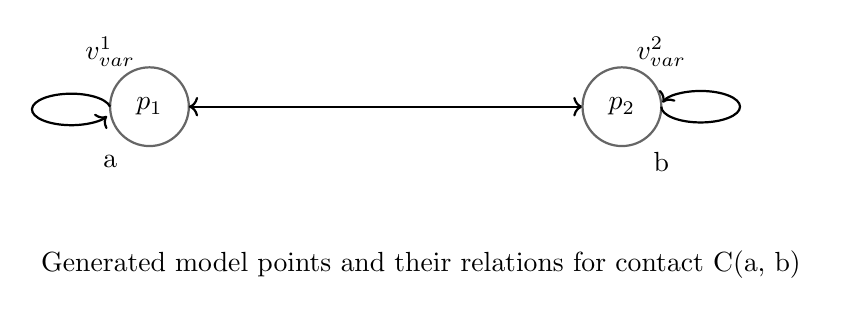
\begin{tikzpicture}[scale = 1]
		\filldraw[color=black!60, fill=red!0, thick](-3,0) circle (0.5);
		\node at (-3.5,0.7) {$\vVar^1$};
		\node at (-3,0) {$p_1$};
		\node at (-3.5,-0.7) {a};
		\draw[thick, ->] (-3.5,0) arc [
      	  		start angle=10,
		       end angle=335,
        		x radius=0.5cm,
        		y radius =0.2cm
    			] ;
		\draw[thick, <->](-2.5,0) -- (2.5,0);
		\filldraw[color=black!60, fill=red!0, thick](3,0) circle (0.5);
		\node at (3.5,0.7) {$\vVar^2$};
		\node at (3,0) {$p_2$};
		\node at (3.5,-0.7) {b};
		\draw[thick, ->] (3.5,0) arc [
      	  		start angle=180,
		      end angle=525,
        		x radius=0.5cm,
        		y radius =0.2cm
    			] ;
		\node[text width=10cm, anchor=west, right] at (-4.5,-2)
    		{Generated model points and their relations for contact C(a, b)};
      \end{tikzpicture}
	\end{center}

	\begin{defn}
		Let B be a branch conjunction and $a \neq 0 \in B$, where a is a term. Then one model point p is generated and its variable valuations $\vVar$ such that:
		\begin{itemize}
			\item $\vBool(a) = \textbf{true}$
		\end{itemize}
		The R relations is extended as follows:
		\begin{itemize}
			\item $pRp$ - reflexivity of the modal point $p$
		\end{itemize}
	\end{defn}
	\leavevmode\newline
	The constructed point diagram:
	\begin{center}
	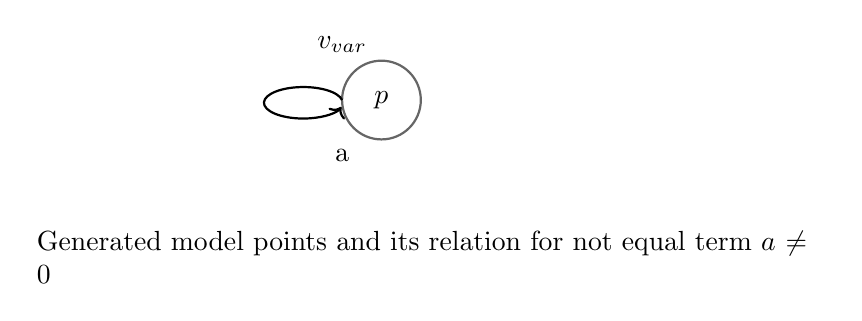
\begin{tikzpicture}[scale = 1]
		\filldraw[color=black!60, fill=red!0, thick](-0,0) circle (0.5);
		\draw[thick, ->] (-0.5,0) arc [
      	  		start angle=10,
		       end angle=345,
        		x radius=0.5cm,
        		y radius =0.2cm
    			] ;
		\node at (-0.5,0.7) {$\vVar$};
		\node at (-0,0) {$p$};
		\node at (-0.5,-0.7) {a};
		\node[text width=10cm, anchor=west, right] at (-4.5,-2)
    		{Generated model points and its relation for not equal term $a \neq 0$};
      \end{tikzpicture}
	\end{center}

	\begin{defn}
		Let B be a branch conjunction and $a \le_\mu b \in B$, where a and b are two terms.
		Then one model point p is generated and its variable valuations $\vVar$ is the constant true, namely the constant term 1.
	\end{defn}
	% say that the meassure atmoic formulas produce one model point 

	\begin{defn}
		With definitions (1, 2, 3) we are able to construct a model where the contacts and non zero terms are satisfied. 
		We will denote this model as \textbf{partially constructed model}. 
		However to satisfy a branch conjunction B we need to verify that the non contacts and zero terms are satisfied as well.
	\end{defn}

	\begin{defn}
		Let M = (W, R) be a partially constructed model. Then we say that the model M satisfies a equal to zero term $a = 0$, if the following holds:
		\begin{align*}
			\forall p \in W: \vBool(a) = \textit{true}
		\end{align*}
	\end{defn}

	\begin{defn}
		Let M = (W, R) be a partially constructed model. Then we say that the model M satisfies a non contact $\neg C(a, b)$, if the following holds:
		\begin{align*}
			\forall p \in W: \vBool(a) = \textit{false} \lor \vBool(b) = \textit{false} \\
			\\
			\forall (p, q) \in R: vBool(p, a) = \textit{false} \lor vBool(q, b) = \textit{false} \\ 
				\land \; vBool(p, b) = \textit{false} \lor vBool(q, a) = \textit{false}
		\end{align*}
	\end{defn}

	\subsection{Sistemi linejni neravenstva} 
		Intro about such systems.

	\subsection{Modeling of a quantitative contact logic formula}
		opisvane na algoritama.

	\newpage
	\section{Implementation Introduction}

	\newpage
	\section{Tableaux Implementation}

	\newpage
	\section{Model Implementation}

	\newpage
	\section{Quantative Contact Logics Implementation}
	
	
% make the vBool with two parameters





























\end{document}
